\chapter{Grundlagen}\label{sec:Chapter2}
In diesem Kapitel werden Grundlagen eingeführt, die für das Verständnis der Evaluation essenziell sind. Im Abschnitt 2.1 werden die theoretischen Grundlagen von DP erläutert. Diese umfassen zum einen das Konzept von \gls{dp} und zum anderen die Metriken für dessen Evaluierung. Im nächsten Abschnitt 2.2 folgt die Vorstellung der drei Frameworks, welche dieses Konzept umsetzten. 
\section{Theorie}
Es werden die Konzepte von \gls{dp} und seine dahinter arbeitenden Mechanismen erläutert. Anschließend folgen verschiedene mathematische Metriken in den drei Kategorien Privatsphäre, Genauigkeit und Erwartungstreue, welche zum Bewerten dieser Eigenschaften eingesetzt werden.
\subsection{Differential Privacy und seine Erweiterung}
Nachdem bestehende Verfahren wie k-anonymity keinen nachweisbar hinreichenden Schutz der Privatssphäre sicherstellten, hat Cynthia Dwork 2006 die mathematische Definition von \gls{dp} veröffentlicht \parencite{DPandSS2020}. Sie lautet: 

Sei $\epsilon$ eine reelle Zahl und $\mA : \mD\longrightarrow\mathcal{S}$ ein gegebener randomisierter Mechanismus mit der Eingabe eines Datensatzes und $S$ als seine Ausgabe. Der Mechanismus garantiert $\epsilon$-differential privacy, wenn für alle Datensätze $\mD_{1}$ und  $\mD_{2}$, welche sich nur in einem Eintrag unterscheiden und alle Untermengen $\mS \in \mathcal{S}$ gilt:
\begin{equation*}
	\Pr\Bigl[ \mA\Bigl( \mD_{1} \in \mS \Bigr) \Bigr]\leq  e^{\epsilon} \cdot \Pr\Bigl[ \mA\Bigl( \mD_{2} \in \mS \Bigr) \Bigr]
\end{equation*}
\parencite{Seminar2017}

Hierbei gilt $\epsilon$ als \gls{pb} und stellt ein Maß für die Privatsphäre dar. Je kleiner der Parameter $\epsilon$ ist, desto mehr werden die Daten privatisiert und desto weniger Informationen lassen sich aus den Daten ablesen. Dabei besteht das Potenzial, dass die Ausgabedaten nicht mehr für den ursprünglichen Zweck nutzbar sind.

\textbf{Beispiel der Gefahr ohne \gls{dp}: }
Anhand der Tabelle \cref{fig:age_cancer_9} und \cref{fig:age_cancer_10} soll durch ein Beispiel \parencite{AlgoFoundations2014} die Gefahr ohne die mathematische Definition von \gls{dp} verdeutlicht werden.

\begin{figure}[htbp]
	\centering
	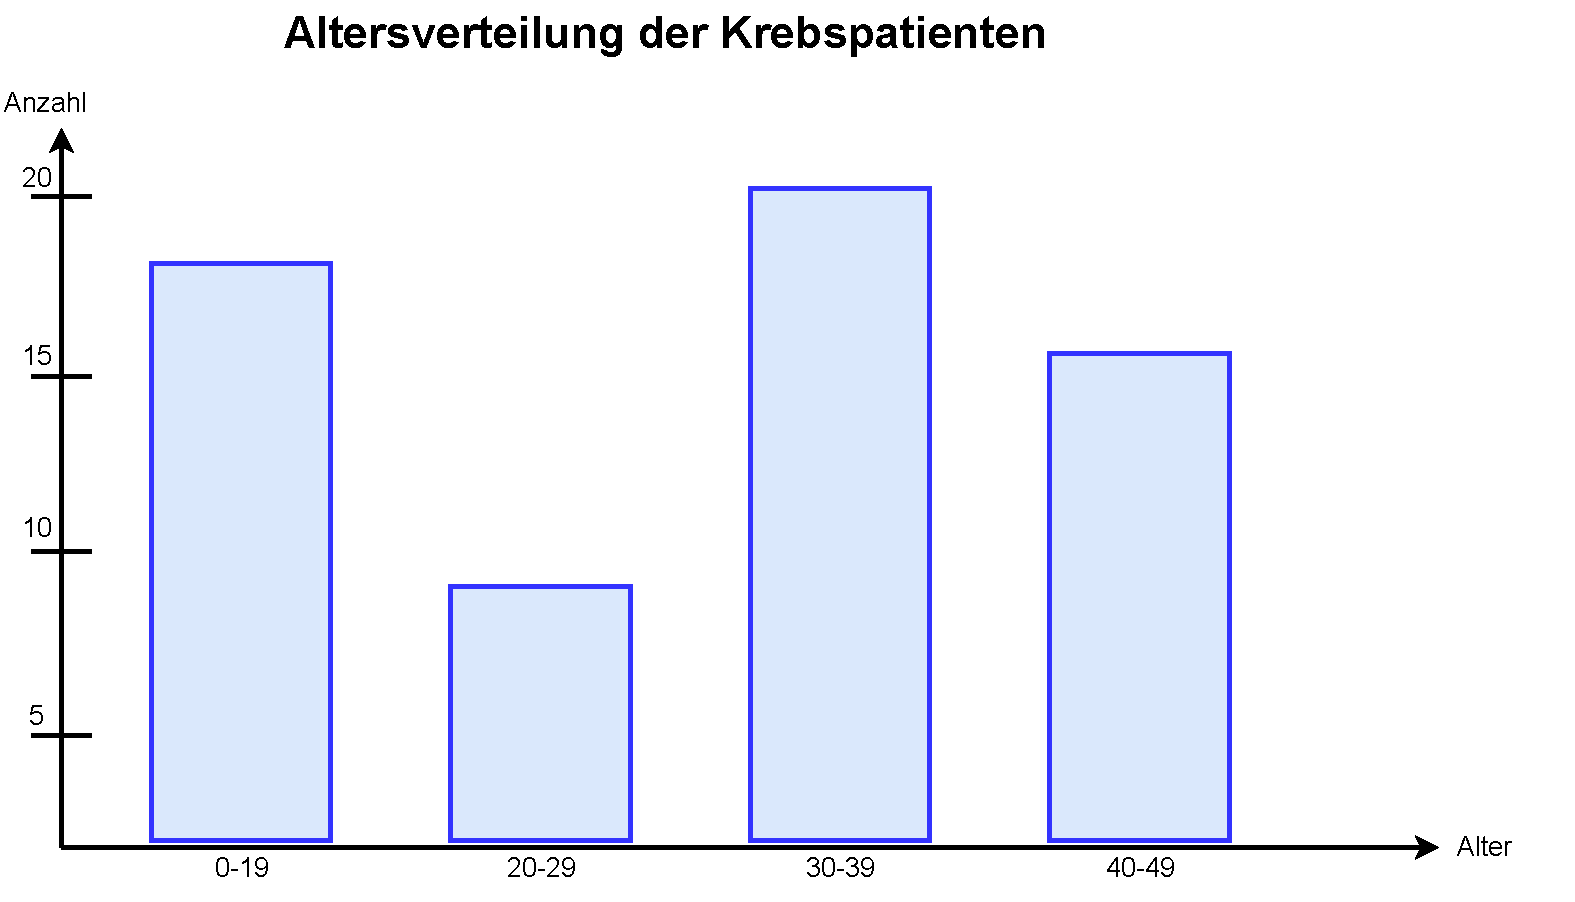
\includegraphics[scale=0.4]{./images/age_cancer_9.pdf}
	\caption{Die Anzahl der Krebspatienten am 12.12.21.}
	\label{fig:age_cancer_9}
\end{figure}
\begin{figure}[htbp]
	\centering
	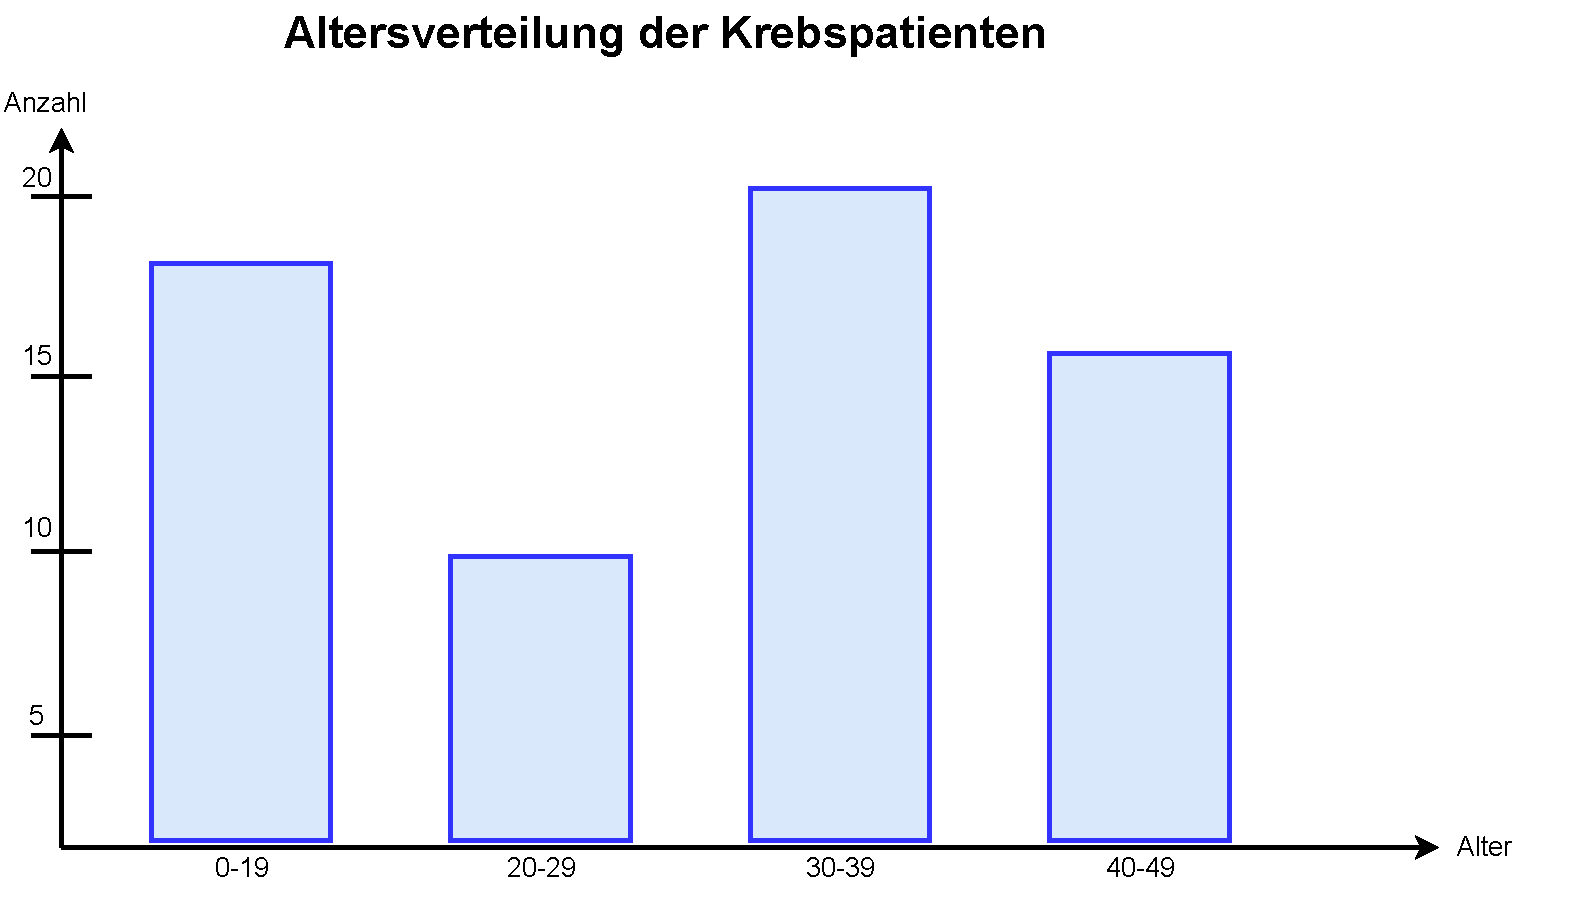
\includegraphics[scale=0.4]{./images/age_cancer_10.pdf}
	\caption{Die Anzahl der Krebspatienten am 13.12.21.}
	\label{fig:age_cancer_10}
\end{figure}

Ein Krankenhaus veröffentlicht täglich seine Statistik zu seiner Anzahl an krebskranken Patienten. Am 12.12.21 veröffentlicht es seine Statistik wie in \cref{fig:age_cancer_9} zu sehen ist. Sie gibt die Anzahl der Kranken nach ihrem Altersintervall an. So ist zum Beispiel die Anzahl der krebskranken Menschen im Alter von 20 bis 29 (inklusive) genau 9 Patienten. Diese Veröffentlichung ist nicht privatisiert und entspricht den tatsächlichen Werten. 

Wenn nun ein Freund Max wissen möchte, ob sein Bekannter Markus an Krebs leidet, dann muss er folgendes mindestens Wissen. Wie alt Markus ist und wann er in dieses Krankenhaus besucht hat. Wenn nun für Markus gilt, dass er 24 Jahre alt ist und am 13.12.21 im Krankenhaus war, dann folgt folgendes. Durch den Vergleich der Tabelle \cref{fig:age_cancer_9} und \cref{fig:age_cancer_10} im Altersintervall 20 bis 29 erfolgt aus der Differenz (10-9), dass eine zusätzliche Person erkrankt ist. Dies trifft dann auf Markus zu, sodass sein Freund Max nun weiß, dass Markus an Krebs erkrankt ist. Die Privatsphäre von Markus ist somit verletzt worden.

\textbf{Erweiterung von \gls{dp}: }
\gls{dp} kann um den additiven Parameter $\delta$ erweitert werden, sodass die Voraussetzungen, dass Informationen versehentlich durchsickern, bis zu einem gewissen Grad $\delta$ unerfüllt bleiben \parencite{Seminar2017}. Die Rückführung der Daten auf die originalen ist verhindert, wenn $\delta$ klein gewählt wird. Der Wert für $\delta$ hängt von der Größe der Datenbank ab. Diese Erweiterung heißt $(\epsilon,\delta)$- Differential Privacy und ist wie gefolgt definiert:
\begin{equation*}
	\Pr\Bigl[ \mA\Bigl( \mD_{1} \in \mS \Bigr) \Bigr]\leq  e^{\epsilon} \times \Pr\Bigl[ \mA\Bigl( \mD_{2} \in \mS \Bigr) \Bigr] + \delta
\end{equation*}
Ein randomisierter Mechanismus $\mA : \mD\longrightarrow\mathcal{S}$ mit der Eingabe eines Datensatzes sei gegeben, welcher alle potenziellen Ausgaben $S$ berechnet. Hierbei sind $\mD_{1}$ und  $\mD_{2}$ beliebige Datensätze, welche sich nur in einem Eintrag unterscheiden. Des Weiteren gilt für alle Untermengen $\mS \in \mathcal{S}$.

\subsection{Laplace Mechanismus}
Ein Mechanismus dient als randomisierter Algorithmus von \gls{dp}, um durch seine Funktion mathematisches Rauschen zu erzeugen. Dieses addierte Rauschen bewirkt das Abändern der Originalwerte im Rahmen der Vorgabe.

Der Laplace Mechanismus basiert auf der Laplace Verteilung wie in \cref{fig:fig_laplace_dib} veranschaulicht. Dieser Mechanismus berechnet das hinzugefügte Rauschen der Daten, um sie durch die Einhaltung von \gls{dp} zu privatisieren. Dafür spielt ebenfalls die Sensibilität \parencite{Seminar2017} der Daten eine Rolle, weswegen sie zuerst erklärt wird.

Sei $\mD$ ein Datensatz und $f: \mD \longrightarrow \mathbb{R}$ eine reellwertige Funktion. Die Sensibilität einer Funktion bezeichnet mit $\Delta f$ ist definiert als: 
\begin{equation*}
	\Delta f = \max |f(x) - f(y)|
\end{equation*}\parencite{AlgoFoundations2014}
wobei das Maximum von allen Paaren des Datensatzes $x$ und $y$ in $\mD$ genommen werden, welche sich nur in einem Eintrag unterscheiden.

Die Sensitivität einer Funktion $f$ gibt das Ausmaß an, wie sehr im schlimmsten Fall die Daten durch ein einzelnes Individuum verändert werden kann und damit die erforderliche eingeführte Veränderung der Antwort, um die Beteiligung einer einzelnen Person zu verbergen.
Durch die Sensitivität einer Funktion wird eine Obergrenze angesetzt, welche ein Maß angibt, wie stark die Ausgabe verrauscht werden muss, um die Privatsphäre zu bewahren.
\pgfmathdeclarefunction{laplace}{2}{%
	\pgfmathparse{1/(2*#2)*exp(-abs(x-#1))/#2)}%
}
\begin{figure}[htbp]\centering
	\begin{tikzpicture}
		\begin{axis}[every axis plot post/.append style={
				mark=none,domain=-3:3,samples=500,smooth,at={(0,0)},
				anchor=north east},
			axis x line*=bottom,
			axis y line*=middle, 
			enlargelimits=upper] 
			\legend{$\mu=0$ $b=1$,$\mu=0$ $ b=2$,$\mu=0$ $ b=4$}
			\addplot {laplace(0,1.0)};
			\addplot {laplace(0.0,2.0)};
			\addplot {laplace(0.0,4.0)};
		\end{axis}
	\end{tikzpicture}
	\caption{Die Laplace Verteilung um den Punkt ($0$,$0$) zentriert.}
	\label{fig:fig_laplace_dib}
\end{figure}

Auf Grundlage der Laplace-Verteilung wie in \cref{fig:fig_laplace_dib} veranschaulicht wird das Rauschen berechnet. Für ihre Dichtefunktion wird zum einen der Parameter $\mu$, welcher für die Lokalität gilt, und zum anderen $b$, welcher zur Skalierung dient, benötigt. Im Falle dieses Mechanismus ist der Parameter $b$ durch $\epsilon$ bestimmt und am Punkt $0$ für $\mu$ zentriert. Dies entspricht der symmetrischen Version der Exponentialverteilung. Eine Zufallsvariable $X$ ist Laplace verteilt, wenn gilt $X \sim Lap(b)$.

Der Laplace Mechanismus berechnet das zufällige Rauschen zu jedem Eintrag im Datensatz. Dazu wird den einzelnen Einträgen in der Antwort zu einer Anfrage $f$ Rauschen nach der Laplace-Verteilung hinzugefügt. Die Definition lautet:
\begin{equation*}
	\mM_{Lap} (x,f,\epsilon) = f(x) + Lap\Biggl(\mu = 0, b = Lap(\frac{\Delta f}{\epsilon})\Biggr)
\end{equation*}
wobei die $X_{i}$ Zufallsvariablen der Laplace-Verteilung $Lap(\frac{\Delta f}{\epsilon})$ sind.


\textbf{Beispiel Histogramm Anfragen: }
Bei solch einer Anfrage wird das Universum $\mathbb{N}^{|X|}$ in Zellen partitioniert \parencite{AlgoFoundations2014}. Die Anfrage fragt nach der Anzahl der Datenbankelementen, die in jeder der Zellen liegen. Aufgrund der disjunkten Zellen steigt bzw. verringert sich die Anzahl der Datenbankelementen nur um eins, wenn eines hinzugefügt oder gelöscht wird. Die Differenz dieser Zelle ist zu den anderen genau $1$, somit hat die Anfrage die Sensibilität von $\Delta f$ = $1$. Bei einer Anfrage kann hiermit zu allen wahren Werten der Zellen das Rauschen unabhängiger Ziehungen aus $Lap(\frac{1}{\epsilon})$ hinzugefügt werden.


\textbf{Beispiel der Funktionalität: }
Die Variable $k$ bezeichnet die Anzahl der Personen mit einer grünen Augenfarbe in der Datenbank \parencite{DPEasy2018}. Nun sei der wahre Wert $k$, welcher nicht veröffentlicht werden kann. Denn sonst kann ein Angreifer dies mit seinem Wissen abgleichen und herausfinden, ob $k-1$ (die Zielperson hat grüne Augen) oder $k$ (die Zielperson hat keine grüne Augen) gilt. Dafür muss er nur die Anzahl der Personen mit grünen Augen aus seinem Wissen mit den der Datenbank vergleichen. 

Für die Privatisierung der Zahl wird Rauschen hinzugefügt und nun wird $k$ = 1003 veröffentlicht. Dagegen ist für dieses Beispiel der wahre Wert $k$= 1001.
Aus der Sicht des Angreifers stellt sich die Frage, mit welcher Wahrscheinlichkeit die originale Zahl 1000 oder 1001 ist. Diese Werte werden mit ihrem zugrundeliegenden Verrauschen in \cref{fig:k_value} gezeigt. Die Hypothese besagt $k$ =1001 ist wahrscheinlicher, denn es ist zutreffend ein Rauschen von Distanz 2 (1003-1001) anstatt 3 (1003-1000) zu erzeugen. Die Abschätzung des Angreifers wird schwieriger desto kleiner $\epsilon$ ist.

\begin{figure}[htbp]
	\centering
	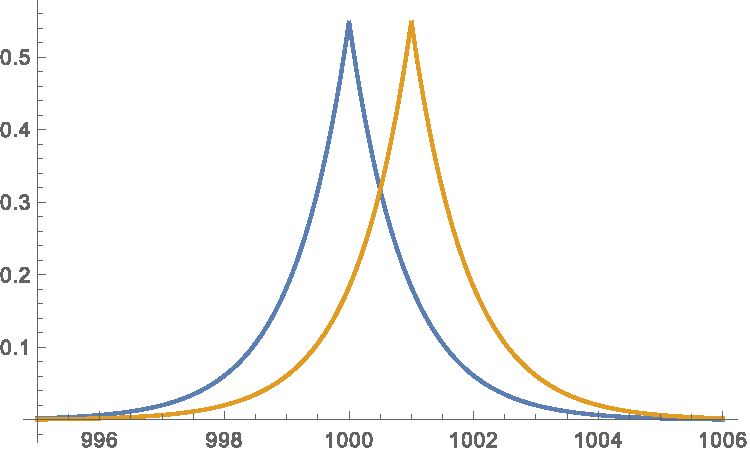
\includegraphics[scale=0.7]{./images/k_laplace_small_eps.pdf}
	\caption{Der wahre Wert ist k=1000 (die blaue Linie) oder k=1001 (die gelbe Linie) \parencite{DPEasy2018}}
	\label{fig:k_value}
\end{figure}

Somit wird dem Angreifer die Zuordnung eines Wertes durch die Überlappung der verschiedenen Laplace Verteilungen erschwert. Bei einem kleineren $\epsilon$ Wert folgt eine größere Abflachung der Verteilungen. 


\subsection{Gauß Mechanismus}
Analog zum Laplace Mechanismus, berechnet der Gauß Mechanismus das Rauschen basierend auf der Gauß Verteilung \parencite{AlgoFoundations2014}. Die Varianz ist von den Parametern für die Privatisierung und der Sensibilität abhängig.

Für beliebige Werte von $\delta \in (0,1)$ und $\epsilon \in (0,1)$ ist der Gauß Mechanismus wie folgt definiert:
\begin{equation*}
	\mM_{Gauss} (x,f,\epsilon,\delta) = f(x) + \mathcal{N}\Biggl(\mu = 0, \sigma^2 = \frac{2\ln(\frac{1.25}{\delta}) (\Delta f)^2}{\epsilon^2} \Biggr)
\end{equation*}

Die Besonderheit bei diesem Mechanismus liegt darin, dass er $(\epsilon,\delta)$-\gls{dp} garantiert, falls $\epsilon < 1$  erfüllt ist. Des Weiteren ist für diesen Mechanismus der Parameter $\delta$ notwendig.

\subsection{Weiterer Mechanismus}
Ein weiterer Mechanismus ist der \gls{rr}, welcher Rückschlüsse auf einzelne Personen verhindern soll \parencite{Seminar2017}. Dies wird hauptsächlich in sozialwissenschaftlichen Studien genutzt, um den Teilnehmer die Möglichkeit zu bieten, brisante Fragen ehrlich beantworten zu können. Aufgrund der verschiedenen Varianten von Randomized Response wird hier die gängigste Variante erklärt, welche auf einem Münzwurf basiert

\begin{figure}[htbp]
	\centering
	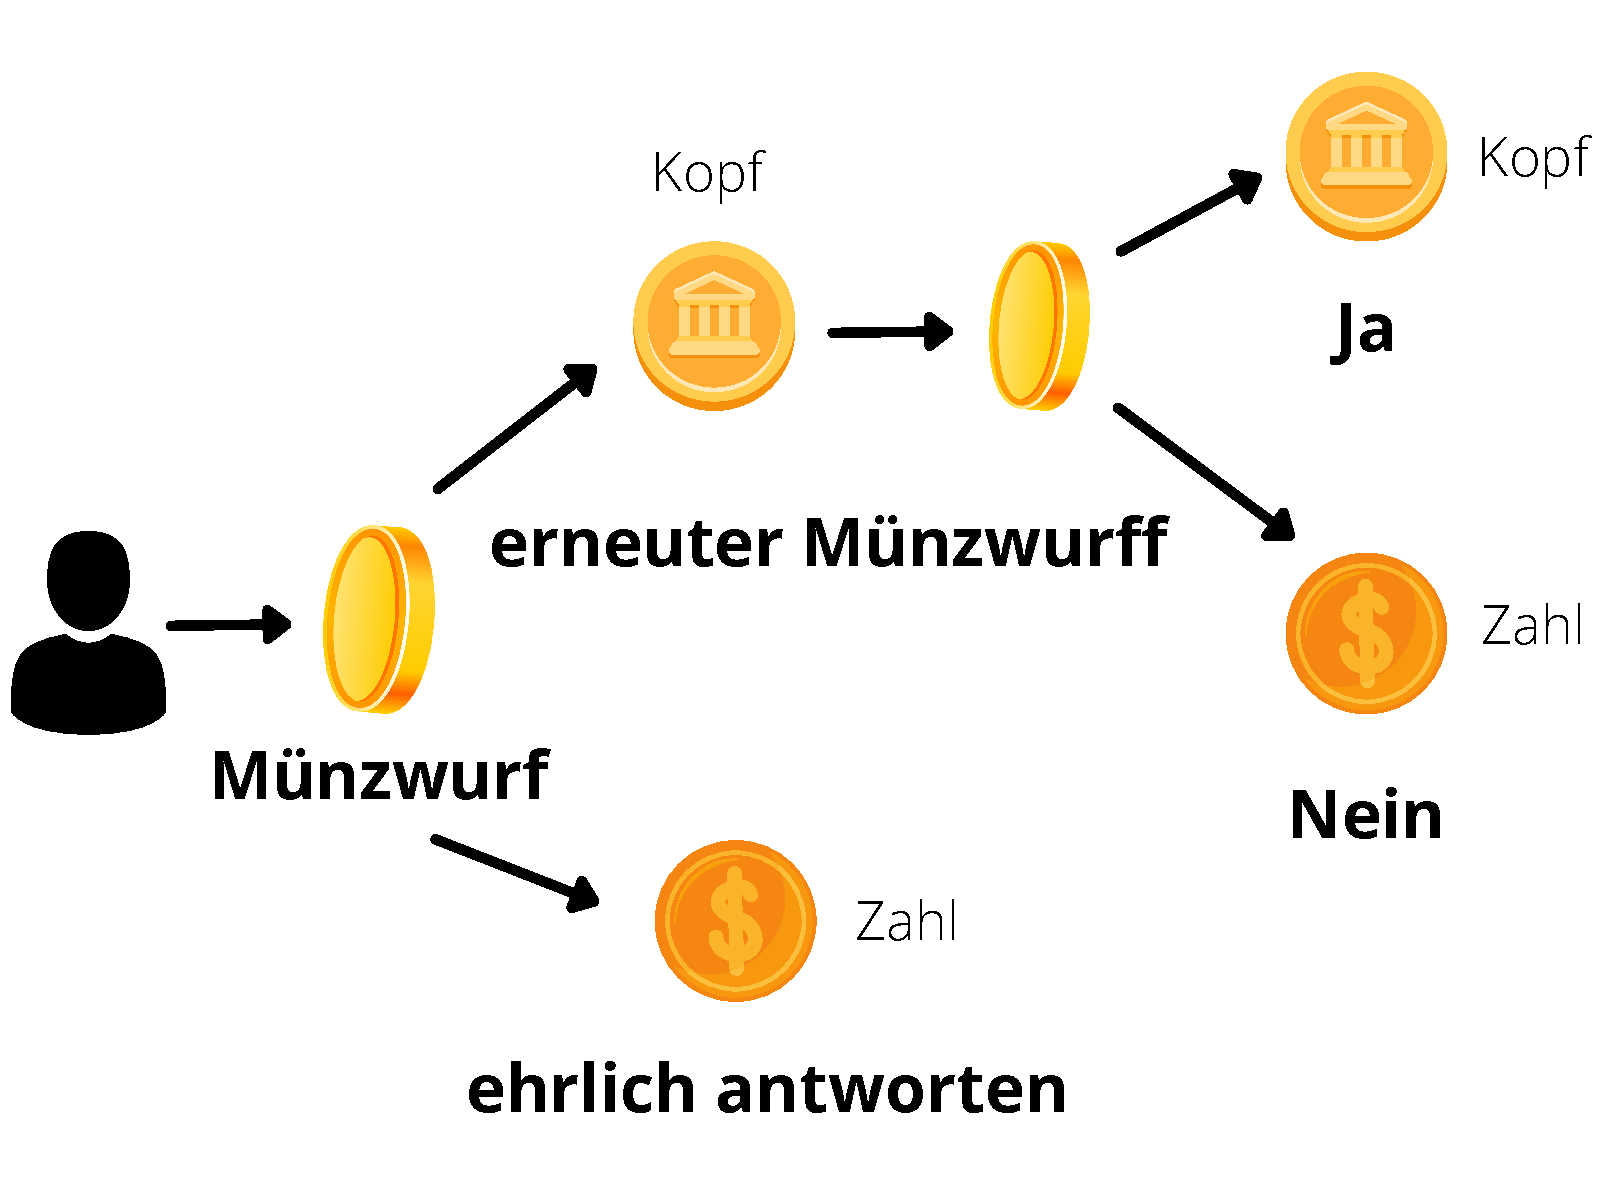
\includegraphics[scale=0.3]{./images/throw_coint.pdf}
	\caption{Eine Veranschaulichung der Entscheidung eines Befragten nach dem \gls{rr} Mechanismus.}
	\label{fig:rr_image}
\end{figure}

Der Befragte wirft eine Münze und folgt der Anweisung wie in Abbildung \cref{fig:rr_image} beschrieben. Wenn die Person beim ersten Wurf eine Zahl erhält, dann beantwortet sie die Frage ehrlich, sonst wirft sie die Münze noch einmal. Beim zweiten Wurf folgt bei Zahl die Beantwortung der Frage mit Nein, sonst mit Ja.

Die Intuition hinter diesem Mechanismus ist, dass dieser Abstreitbarkeit unterstützt. Wenn die Frage z.B. mit \enquote{Ja} beantwortet wurde, kann dies aufgrund des ersten und zweiten Wurfs, welche Kopf waren, geschehen sein. Die dazugehörige Wahrscheinlichkeit beträgt dann $\frac{1}{4}$. 
Es bleibt also ungewiss, ob die Person die Frage ehrlich beantwortet oder ob sie die Antwort der Münze wiedergibt. 
Dieser Prozess lässt eine Interpretation der Antworten zu, da die Art und Weise wie die Antworten eingeholt werden, nicht eindeutig nachvollziehbar sind.

Bei solchen Zufallsexperimenten wie dem Münzwurf nähert sich das Ergebnis bei häufiger Wiederholung dem erwarteten. Somit kann man davon ausgehen, dass die Hälfte der Antworten ehrlich angegeben worden sind. Dieser Mechanismus erfüllt \gls{dp}, genauer $\epsilon = ln(3)$.

\subsection{Privatsphäre-Metriken}
Im Bereich der Privatsphäre dienen die Metriken DP-res und Wasserstein Distanz als Messwert, inwieweit die Definition von \gls{dp} eingehalten wird und wie gut die Qualität des Verrauschens ist. Zum einen prüft die Metrik DP-res die Einhaltung von \gls{dp} nach und zum anderen die Metrik Wasserstein Distanz misst die Verschiedenheit der Datensätze nach dem Verrauschen.

\paragraph{DP-res (($\epsilon$,$\delta$)-DP begrenztes Histogramm Test)}
Dies ist ein $(\epsilon, \delta)$ \gls{dp} Histogramm Test aus dem Framework smart-noise-eval (siehe Kapitel 2.2) für benachbarte Datensätze D1 und D2. Das Ergebnis ist entweder wahr oder falsch.
Hierfür werden die beiden Datensätze durch die Ausführung einer Funktion (z.B. Durchschnittsfunktion) in angegebener Häufigkeit berechnet. Aus den aggregierten Daten wird zunächst ein Histogramm erzeugt. Anschließend folgt der Test der Histogramme, ob sie \gls{dp} einhalten. In diesem Test werden die Werte des Histogramms des erste Datensatzes mit $e^\epsilon$ multipliziert und mit $\delta$ summiert, wobei überprüft wird, ob das Histogramm in den Grenzen des zweiten Datensatzes liegt. Ebenfalls erfolgt dies umgekehrt.

\textbf{Interpretation für \gls{dp}: }
Das Ergebnis des Testes sagt aus, inwieweit die Definition von \gls{dp} eingehalten wurde. Wenn das Ergebnis wahr ist, dann ist es gültig, sonst nicht.
\paragraph{Wasserstein-Distanz}
Die Wasserstein-Distanz \parencite{WDExplanation} ist ein Maß um die Distanz zwischen zwei Wahrscheinlichkeitsverteilungen zu berechnen. Sie wird auch als \enquote{Earth Mover's distance} in der Dimension 1 bezeichnet. Dieser Name folgt aus der Interpretation von ihr als das Minimum der Energiekosten für das Verschieben und Transformieren eines Erdhaufens in Form einer Wahrscheinlichkeitsverteilung in die Form der anderen Verteilung. Für diese Bachelorarbeit wird die erste Dimension der Distanz benötigt, sodass sie als numerische Metrik genutzt werden kann. In der \cref{fig:wd} wird diese Interpretation veranschaulicht. Die kleinen blauen und roten markierten Stellen des Graphen sollen ineinander überführt werden. Dafür wird zum einen durch den Pfeil die Distanz gekennzeichnet und zum anderen die Wahrscheinlichkeit für die Umformung beachtet.


Die Distanz zwischen zwei diskreten Distributionen $f$ und $g$ ist wie folgt definiert:
\begin{equation*}
	\mW_{1} (f,g) = \inf_{h \in \mH(\mX,\mY|f,g)} \mE_{(x,y)\sim h} \Bigl[|\mX - \mY|\Bigr]
\end{equation*}
Hierbei ist $\mH$ eine Menge von allen vereinten Verteilungen der Variablen $\mX$ und $\mY$, welche die marginale Verteilungen $f$ und $g$ haben.
\begin{figure}[htbp]
	\centering
	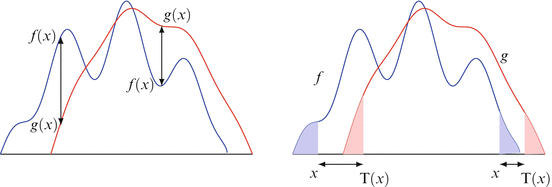
\includegraphics[scale=0.4]{./images/wasserstein_distance.png}
	\caption{Der Transport von $x$ nach $\mT(x)$ und andersherum wird mit der $\mW_{1}$ im rechten Bild berechnet, wobei die Flächen von f und g gleichgesetzt werden. \parencite{Santambrogio2015}}
	\label{fig:wd}
\end{figure}

Eine intuitive Interpretation dieser Metrik ist die Summe der Flächen zwischen zwei kumulativen Dichtefunktionen. Wenn $\mF(x)$ und $\mG(x)$ die kumulativen Dichtefunktionen von $f(x)$ und $g(x)$ sind, dann kann $\mW_{1}$ auch definiert werden als:

\begin{equation*}
	\mW_{1} (f,g) = \int_{\infty}^{\infty} |\mF(x) - \mG(x)| dx
\end{equation*}
\parencite{WDDef}
Die Wasserstein-Metrik ist eine echte Wahrscheinlichkeitsmetrik und berücksichtigt sowohl die Wahrscheinlichkeit als auch den Abstand zwischen verschiedenen Ergebnisereignissen.

\textbf{Interpretation für \gls{dp}: }
Diese Metrik kann sehr gut für die numerische Ähnlichkeit der originalen und verrauschten Daten eingesetzt werden. Des Weiteren kann der Wert der Metrik in Bezug für verschiedene $\epsilon$- Werte zur Veranschaulichung der Hinzunahme von Rauschen verwendet werden. Somit kann die Qualität der Frameworks in der Berechnung des Rauschens verglichen und ausgewertet werden.

\subsection{Genauigkeits-Metriken}
Im Bereich der Genauigkeit diene die Metriken die mittlere quadratische Abweichung und Standardabweichung als Messwerte, inwieweit das Verrauschen auf die Qualität der Genauigkeit einen Einfluss hat. Bei niedrigen $\epsilon$ Werten ist eine große Ungenauigkeit zu erwarten, bei großen soll das Gegenteil zutreffen.
\paragraph{Mittlere quadratische Abweichung}
Die mittlere quadratische Abweichung (in Englisch \gls{mse}) \parencite{MSE2022} gibt an, wie sehr ein Punktschätzer um den zu schätzenden Wert streut.
Wenn eine geringe mittlere quadratische Abweichung gilt, dann folgt gleichzeitig ein kleiner Bias und eine kleine Varianz des Schätzers. Der Schätzer liegt somit im Mittel in der Nähe des zu schätzenden Funktionals (kleiner Bias) und die Schätzwerte streuen wenig (kleine Varianz). Die Wahrscheinlichkeit, dass Schätzwerte in der Nähe ihres Erwartungswertes liegen, ist somit groß.

Ihre Definition lautet:

Sei $\mathcal{Y}$ der Vektor der beobachteten Werte und $\grave{\mathcal{Y}}$ der Vektor der vorhergesagten Werte. Der Vektor von $n$ Vorhersagen wird durch eine Stichprobe mit $n$ Datenpunkten aller Variablen und der vorherigen Vektoren generiert. Innerhalb der Stichprobe wird die mittlere quadratische Abweichung wie folgt berechnet:
\begin{equation*}
	MSE = \frac{1}{n} \sum_{i=1}^{n} (\mathcal{Y}_{i} -\grave{\mathcal{Y}}_{i})^2
\end{equation*}

\textbf{Interpretation für \gls{dp}: }
In Kontext von \gls{dp} kann anhand der mittleren quadratischen Abweichung die Genauigkeit der verrauschten Daten berechnet werden. Dafür gelten die originalen Daten der Funktion (z.B. der Durchschnitt) der tatsächlichen Stichprobe und die vorhergesagten Datenwerten der verrauschten Daten. Wenn das berechnete Resultat nahe an $0$ ist, gilt für die verrauschten Daten eine hohe Genauigkeit.

\paragraph{Standardabweichung}
Wenn die Quadratwurzel der Varianz genommen wird, dann ist der entsprechende Wert die Standardabweichung \parencite{SDLexikon} , welche als eines der wichtigsten Streuungsmaße in der Stochastik gilt.
Die Varianz ist definiert als die zu erwartende quadratische Abweichung einer Zufallsvariable zu ihrem Erwartungswert. Dagegen ist die Standardabweichung die durchschnittliche Entfernung aller gemessenen Daten vom Durchschnitt.

Wenn die Standardabweichung \parencite{SDNormalverteilung} der Daten berechnet wird, liefert sie die Information, wie weit sich diese Daten zwischen dem Minimum und dem Maximum verteilen, vor allem wie dicht sie sich um den Mittelwert häufen. Die Verteilung der Datenpunkte kann in einer Kurve dargestellt werden, welche meistens die Form einer Glocke hat. Dies wird in \cref{fig:nv_std} deutlich. Die Werte liegen entsprechend der Normalverteilung vor und die Standardabweichung zeigt die räumliche Distanz zum Mittelwert.

Sei $\mX$ eine Zufallsvariable und ihr Erwartungswert $\mathbb{E}(X)=\mu$, dann ist die Standardabweichung \parencite{Varianz}:
\begin{equation*}
	SD(\mX) := +\sqrt{VAR(\mX)} = +\mathbb{E}((\mX-\mu)^2)
\end{equation*}
Auch als $\sigma_{x}$ bezeichnet.

\begin{figure}[htbp]
	\centering
	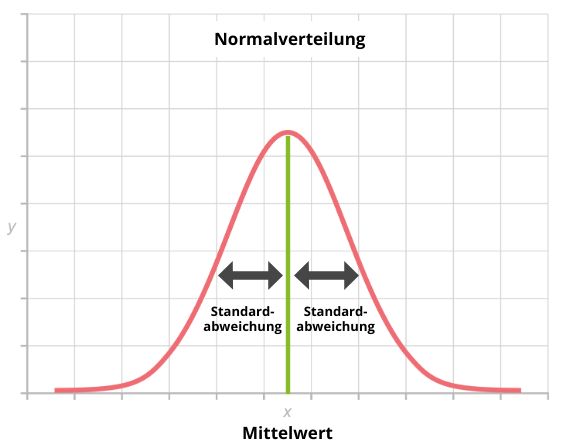
\includegraphics[scale=0.7]{./images/standard_deviation.png}
	\caption{Die Funktionalität der Standardabweichung. \parencite{STD}}
	\label{fig:nv_std}
\end{figure}

\textbf{Interpretation für \gls{dp}: }
In Kontext von \gls{dp} kann anhand der Standardabweichung bestimmt werden, inwiefern die Ausgabe durch das Rauschen des Laplace Mechanismus streut. Wenn die Standardabweichung klein ist, dann unterscheiden sich die verrauschten Ausgaben nicht sehr voneinander. Andersherum gilt dies auch. Dies gilt für den Laplace Mechanismus.

Insbesondere beim Gauß Mechanismus mit seiner Gauß-Verteilung kann eine Normalverteilung vorliegen, sodass sie sich zur Quantifizierung von Unsicherheit bei Entscheidungen unter Risiko eignen kann. In gewissen Intervallen der Standardabweichung ($\pm\sigma_{x}$, $\pm2\sigma_{x}$ usw.) kann die Wahrscheinlichkeit für das Aufkommen der Werte in einem Intervall berechnet werden. Dies kann zur Bewertung des Verrauschens benutzt werden.

\subsection{Erwartungstreue-Metrik}
Im Bereich der Erwartungstreue dient die Metrik mittlere vorzeichenbehaftete Abweichung als Messwert, inwieweit das Verrauschen die Werte verzerrt hat. Desto mehr die Werte verzerrt sind, desto weniger sind sie semantisch nutzbar. Die Aussagekraft der verrauschten Werte gegenüber den originalen verschwindet dadurch.
\paragraph{Mittlere Vorzeichenbehaftete Abweichung}
Die mittlere vorzeichenbehaftete Abweichung wird im Englischen als \gls{msd} bezeichnet.
Es gibt eine Menge von $n$ Paaren ($\theta_{i}$,$\hat{\theta_{i}}$), wobei $\theta_{i}$ für den tatsächlichen Wert und $\hat{\theta_{i}}$ für den geschätzten Wert steht \parencite{MSD}. Die Definition lautet:

\begin{equation*}
	MSD(\hat{\theta_{i}}) := \frac{1}{n} \sum_{i=1}^{n}  \hat{\theta_{i}} - \theta_{i}
\end{equation*}

\textbf{Interpretation für \gls{dp}: }
Bei dieser Metrik wird die Differenz von dem originalen Wert und dem verrauschten Wert paarweise berechnet und davon dann insgesamt der Mittelwert genommen. Dieser Wert veranschaulicht, ob durchschnittlich das Rauschen des Mechanismus zu viel (positiver Wert) oder zu wenig (negativer Wert) war. Somit kann das Verhalten des Mechanismus aufgezeigt und Schlüsse gezogen werden, ob die Informationen in den Daten erhalten bleiben.
\newpage
\section{Technische Aspekte der Frameworks}
In diesem Abschnitt werden die drei Frameworks in ihrer gesamten Struktur erklärt. Dies beginnt mit dem Aufbau des Frameworks bis zu seinen Besonderheiten, die es von den anderen abgrenzt. Zum Schluss folgt eine allgemeine Übersicht des Frameworks für den Einsatz in \gls{dp}.
\subsection{Smartnoise SDK}
\textbf{Technologie: }
Dieses Framework \parencite{Smartnoise}  kann in der Programmiersprache Python genutzt werden. Des Weiteren werden für zusätzliche Funktionalitäten die SQL-Sprache benötigt, um über die bereitgestellten Funktionen hinaus agieren zu können.

\textbf{Aufbau: }
Dieses Framework wird in drei Module smartnoise-sql, smartnoise-synth und smartnoise-eval untergliedert. Jeder dieser Teilbestände ist eine eigene Bibliotheken. Für diese Arbeit ist lediglich smartnoise-sql relevant. In der Teilbibliothek smartnoise-sql werden durch SQL-Anfragen innerhalb der Programmiersprache Python Daten ausgelesen und ihr Ergebnis verrauscht. Die Funktionalität stammt ursprünglich aus der Bibliothek \gls{opendp} \parencite{OpenDP}. Sie ist eine Ansammlung an statistischen Algorithmen, die die Definition von \gls{dp} einhalten. Durch die Anfragen können diese Berechnungen daraus vollzogen werden. 

\textbf{Beschreibung der Funktionen: }
Durch fünf verschiedene Methoden können Daten im Framework eingelesen werden. Unter diesen ist eine Datenbankverbindung möglich. Für das Nachverfolgen des \gls{pb}s steht die Funktionalität \enquote{odometer}(Kilometerstand) zur Verfügung. Während der Auswertung kann die Menge an benötigtem \gls{pb} eingesehen werden. Durch weitere Funktionen der Lesemethode \enquote{readers} kann die durchschnittliche Genauigkeit der Anfragen innerhalb eines Intervalls; z.B. 95\% der Fälle angegeben werden. Für die Veranschaulichung der Daten wird beim Histogramm automatisch Angaben wie der Nachname gelöscht, die die Privatsphäre verletzen könnten.

\textbf{Besonderheit: }
Eine direkte Verbindung zu einer SQL-Datenbank ist durch dieses Framework möglich. Hierbei ist ein unmittelbarer Zugriff auf die Originaldaten nicht von Nöten.

\textbf{Fazit: }
Insgesamt deckt dieses Framework die grundlegenden Funktionen für eine Auswertung durch seine Funktionalitäten ab. Des Weiteren bietet es fünf verschieden Möglichkeiten, um Daten auslesen zu können.

\subsection{IBM DP}
\textbf{Technologie: }
Dieses Framework \parencite{diffprivlib} kann in der Programmiersprache Python genutzt werden. Neben den statistischen Funktionen stehen weitere Funktionen im Bereich des \gls{ml}s zur Verfügung.

\textbf{Aufbau: }
Dieses Framework kann in die vier großen Hauptkomponente Mechanismen, Modelle, Tools und Accountant des \gls{pb}s unterteilt werden. Die Mechanismen besitzen alle grundlegenden Funktionalitäten, welche \gls{dp} nutzen. 
Die Modelle sind für \gls{ml} mit \gls{dp} einsetzbar. Diese lassen sich in Clustering, Klassifizierung, Regression, Dimensionsreduktion und Vorverarbeitung untergliedern. Dagegen stellen die Tools generische Funktionen für \gls{dp} gerechte Datenanalyse an, worin ein verrauschtes Histogramm enthalten ist. Zuletzt kann \enquote{Accountant} zum Nachverfolgen des investierten \gls{pb} verwendet werden. Fortschrittliche Kompositionstechniken berechnen zusätzlich dabei den Verlust an Privatsphäre.

\textbf{Beschreibung der Funktionen: }
Die Funktionalität richtet sich eher nach \gls{ml} und bietet dementsprechend überwiegend solche Methoden an. Diese umfassen grundlegende wie z.B. logistische Regression, k\_means, pca usw. mit Verwendung von \gls{dp}.
Neben dessen können statistische Funktionen wie die Anzahl, Durchschnitt, Summe usw. durch vordefinierte Funktionen aufgerufen werden. Eine Besonderheit liegt darin, \gls{dp} gerechte Histogramme, auch multidimensionale, erzeugen zu können. Zusätzlich kann der Einsatz des \gls{pb}s durch Accountant nachverfolgt werden. Somit stehen dem Forscher die Funktionen in den Bereichen Mechanismen, Modelle, Tools und Accountant zur Einsetzung bereit.

\textbf{Besonderheit: }
Die Mechanismen umfassen auch Funktionen im Bereich des \gls{ml}s. Hierfür werden grundlegende Modelle mit einer verrauschten Ausgabe durch \gls{dp} angeboten.

\textbf{Fazit: }
Insgesamt liegt der Fokus dieses Frameworks eher im Bereich \gls{ml}. Darin sind Modelle vorhanden, die in den Eingaben sowie im Trainieren richtig benutzt werden müssen. Sonst können deren Ergebnisse nicht aussagekräftig sein. Daher richtet sich dieses Framework in diesem Bereich eher an Experten in \gls{ml}, die ihre Ideen umsetzten, möchten. Im Bereich \gls{dp} sind grundlegende Funktionen vorhanden und können für eine Datenanalyse genutzt werden.

\subsection{Google DP}
\textbf{Technologie: }
Dieses Framework \parencite{DPGoogle} kann in der Programmiersprache Java, C++ und Go genutzt werden. Dafür stehen drei verschiedene Block-Bibliotheken, die in den jeweiligen Sprachen die grundlegenden Funktionen für \gls{dp} gerechte Auswertung implementieren, zur Verfügung.

\textbf{Aufbau: }
Die gesamte Bibliothek Google \gls{dp} ist in Tools unterteilt, die verschiedene Anwendungen umfassen.
Für eine einfache Anwendung durch Nicht-Experten kann \enquote{Privacy on Beam} genutzt werden. Dies ist ein End-zu-End \gls{dp} Framework, welches auf Apache Beam gebaut ist. Dafür wird keine Vorkenntnis in \gls{dp} vorausgesetzt. Lediglich die Angabe des \gls{pb}s genügt als Parametrisierung für die Berechnung. Für diese Arbeit ist der \enquote{Stochastische Tester} irrelevant. Wie bei den anderen Bibliotheken ist es möglich, das eingesetzte \gls{pb} nachzuverfolgen. Für eine Anwendung mit der SQL-Sprache bietet dieses Framework die Schnittelle \enquote{ZetaSQL} an. Sie verfügt die Eingabe von Anfragen durch SQL und und stellt dafür eine Kommandozeilen-Schnittstelle bereit.

\textbf{Beschreibung der Funktionen: }
Durch die fertig implementierten Block-Bibliotheken werden jeweils 14 Funktionen von statistischen, wie z.B. der Durchschnitt, bis zu graphisch basierenden Funktionen, wie z.B. \enquote{Laplace thresholding}, bereit gestellt. Darüber hinaus können durch SQL-Anfragen Daten ausgewertet werden.

\textbf{Besonderheit: }
Eine flexible Anwendung dieses Frameworks ist durch die drei verschiedenen Programmiersprachen möglich. Für einen Einstieg in \gls{dp} ist Privacy on Beam geeignet.

\textbf{Fazit: }
Insgesamt liegt der Fokus dieses Frameworks einheitlich auf \gls{dp}. Es stehen verschiedene Anwendungen durch statistische Funktionen zur Verfügung, die in ihrer Funktionalität eingeschränkt sind. Eine übliche Auswertung durch SQL-Anfragen ist ebenfalls möglich.

\newpage
\section{Vergleich}
Eine Gegenüberstellung der Frameworks in verschiedenen Gebieten erfolgt in \cref{tab : compare_frameworks}. Die drei Frameworks stellen grundlegende statistische Methoden für eine Auswertung bereit. Die verwendeten Mechanismen fürs Verrauschen basieren auf den zwei grundsätzlichen und IBM \gls{dp} bietet zusätzlich noch den exponentiellen an.  Zwei der Frameworks sind einzig auf \gls{dp} fokussiert, IBM \gls{dp} umfasst ebenfalls das Thema \gls{ml}. Ein Gebrauch der SQL-Sprache ist außer beim IBM \gls{dp} möglich. Einzig Smartnoise SDK bietet eine Auslesung der Daten aus einer Datenbank an. Bei den restlichen ist dies nur durch Auslesen von CSV Dateien realisierbar. Eine Vielfalt an Programmiersprachen bietet das Google \gls{dp} an, und zwar drei verschiedene. Die anderen beiden können nur in Python eingesetzt werden. Als einziges Framework kann das Google \gls{dp} bei der Eingabe eines Algorithmus validieren, ob er nicht \gls{dp} einhält. Die Entscheidbarkeit des Überprüfers hierbei ist semi-entscheidbar.

\begin{table}[h]
	\centering
	\begin{tabular}{ l l l l} \toprule
		& \textbf{Smartnoise SDK} & \textbf{Google DP} & \textbf{IBM DP}  \\ \midrule
		\textit{bereitgestellte Funktionen}	&  & &\\ \hline
		Laplace Mechanismus	& X  & X & X\\
		Gaussian Mechanismus	& X & X & X\\
		Exponentieller Mechanismus	&  & & X\\
		Summe	&  X & X & X\\
		Varianz   &  X & X & X\\
		Standardabweichung & X & X &X\\
		Anzahl	&  X & X & X\\ \hline
		\textit{Besonderheiten} & & &\\ \hline
		Modelle (\gls{ml})	&  & & X\\ 
		SQL-Anfragen	&  X & X &\\ 
		Auslesungsart der Daten	&  SQL-Sprache&CSV  & CSV\\ 
		Programmiersprache	&  Python& Go, Jave \& C++ & Python\\ 
		DP Algorithmus Validierer	&  & X &\\ \bottomrule
	\end{tabular}
	\caption{Vergleich der Frameworks in ihren Eigenschaften.}
	\label{tab : compare_frameworks}
\end{table}
